


\tikzset{every picture/.style={line width=0.75pt}} %set default line width to 0.75pt        

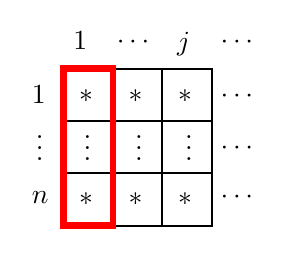
\begin{tikzpicture}[x=0.75pt,y=0.75pt,yscale=-1,xscale=1]
%uncomment if require: \path (0,534); %set diagram left start at 0, and has height of 534

%Shape: Rectangle [id:dp17271303952502315] 
% \draw   (52.81,325.2) -- (76.62,325.2) -- (76.62,350.41) -- (52.81,350.41) -- cycle ;
%Shape: Rectangle [id:dp4366577772656428] 
\draw   (76.81,350.41) -- (100.62,350.41) -- (100.62,375.62) -- (76.81,375.62) -- cycle ;
%Shape: Rectangle [id:dp13823281826780653] 
\draw   (76.81,325.2) -- (100.62,325.2) -- (100.62,350.41) -- (76.81,350.41) -- cycle ;
%Shape: Rectangle [id:dp25508926192152326] 
\draw   (100.62,325.2) -- (124.43,325.2) -- (124.43,350.41) -- (100.62,350.41) -- cycle ;
%Shape: Rectangle [id:dp7615695748694848] 
\draw   (124.43,325.2) -- (148.24,325.2) -- (148.24,350.41) -- (124.43,350.41) -- cycle ;
%Shape: Rectangle [id:dp7082057113045306] 
\draw   (100.62,350.41) -- (124.43,350.41) -- (124.43,375.62) -- (100.62,375.62) -- cycle ;
%Shape: Rectangle [id:dp5459336420864682] 
\draw   (124.43,350.41) -- (148.24,350.41) -- (148.24,375.62) -- (124.43,375.62) -- cycle ;
%Shape: Rectangle [id:dp8229762223203931] 
\draw   (76.81,375.62) -- (100.62,375.62) -- (100.62,400.83) -- (76.81,400.83) -- cycle ;
%Shape: Rectangle [id:dp7425833826219033] 
\draw   (100.62,375.62) -- (124.43,375.62) -- (124.43,400.83) -- (100.62,400.83) -- cycle ;
%Shape: Rectangle [id:dp11427372040336436] 
\draw   (124.43,375.62) -- (148.24,375.62) -- (148.24,400.83) -- (124.43,400.83) -- cycle ;
%Shape: Rectangle [id:dp835448558688529] 
\onslide<2->{\draw  [color={rgb, 255:red, 255; green, 0; blue, 0 }  ,draw opacity=1 ][line width=2.25]  (76.81,325.2) -- (100.62,325.2) -- (100.62,400.83) -- (76.81,400.83) -- cycle ;}

% Text Node
\draw (82.82,334.01) node [anchor=north west][inner sep=0.75pt]    {$*$};
% Text Node
\draw (106.63,334.01) node [anchor=north west][inner sep=0.75pt]    {$*$};
% Text Node
\draw (130.44,334.01) node [anchor=north west][inner sep=0.75pt]    {$*$};
% Text Node
\draw (82.82,383.43) node [anchor=north west][inner sep=0.75pt]    {$*$};
% Text Node
\draw (106.63,383.43) node [anchor=north west][inner sep=0.75pt]    {$*$};
% Text Node
\draw (130.44,383.43) node [anchor=north west][inner sep=0.75pt]    {$*$};
% Text Node
\draw (62,348) node [anchor=north west][inner sep=0.75pt]    {$\vdots $};
% Text Node
\draw (60,332) node [anchor=north west][inner sep=0.75pt]    {$1$};
% Text Node
\draw (60,383) node [anchor=north west][inner sep=0.75pt]    {$n$};
% Text Node
\draw (85,348) node [anchor=north west][inner sep=0.75pt]    {$\vdots $};
% Text Node
\draw (109.81,348) node [anchor=north west][inner sep=0.75pt]    {$\vdots $};
% Text Node
\draw (133.81,348) node [anchor=north west][inner sep=0.75pt]    {$\vdots $};
% Text Node
\draw (80,306) node [anchor=north west][inner sep=0.75pt]    {$1$};
% Text Node
\draw (101,308) node [anchor=north west][inner sep=0.75pt]    {$\cdots $};
% Text Node
\draw (130,306) node [anchor=north west][inner sep=0.75pt]    {$j$};
% Text Node
\draw (151,308) node [anchor=north west][inner sep=0.75pt]    {$\cdots $};
% Text Node
\draw (151,334) node [anchor=north west][inner sep=0.75pt]    {$\cdots $};
% Text Node
\draw (151,359) node [anchor=north west][inner sep=0.75pt]    {$\cdots $};
% Text Node
\draw (151,383) node [anchor=north west][inner sep=0.75pt]    {$\cdots $};
% Text Node
% \draw (57.82,334.01) node [anchor=north west][inner sep=0.75pt]    {$*$};


\end{tikzpicture}
